% sec_game.tex -- Section 5: The abstract game and its soundness (author B)

\section{The abstract game and its soundness}\label{sec:game}

On the empty board no pairing exists (the $148$ lines would need $296$ cells), so \Breaker{} cannot follow a
pairing strategy from the first move. Instead \Breaker{} first places stones according to a finite table until
the leaf certificate $\LEAF(B,F,t)$ of \cref{def:leaf} holds, and plays a pairing strategy from then
on. This section makes the table precise. We define a finite \emph{abstract game} whose states are labeled
\WON{} by a recursion, and \emph{certificates}, which are finite witnesses for the statement that the root of
the abstract game is \WON. From a certificate we define a strategy $\sigma$ for \Breaker{} and prove that
$\sigma$ always prescribes an empty cell and never lets \Maker{} own a whole line
(\cref{thm:soundness,thm:sigma}). Together with a strategy-stealing argument this proves
\cref{thm:main}. Every statement of this section is proved by hand. The existence of a certificate
(\cref{fact:H}) enters only as a hypothesis.

\medskip\noindent\textbf{Conventions.}
Throughout, $B$ and $X$ are disjoint sets of cells: the stones of \Breaker{} and of \Maker. Lines are live
with respect to $B$, and $\live{B}$ is the set of live lines. We write $B+e$ for $B\cup\{e\}$. By
\cref{lem:geometry}\,(c) two distinct lines have at most one common cell; this is used constantly, and
references to \cref{lem:geometry} always mean this statement. We use
the terminology of \cref{def:admissible}: a \emph{threat} of $X$ is a live line with exactly five cells in
$X$; a \emph{danger pair} of $X$ consists of two distinct live lines, each with exactly four cells in $X$,
which share a cell outside $X$ (the \emph{common cell} of the pair); and $X$ is \emph{$B$-admissible} if
$X\cap B=\emptyset$, every live line has at most four cells in $X$, and $X$ has no danger pair. Threats and
danger pairs always refer to the set $B$ under consideration, and both words are used for arbitrary sets
$X$ disjoint from $B$, admissible or not. \cref{lem:adm-closed} is used in the following form: if $X$ is
$B$-admissible, then every subset of $X$ is $B$-admissible (part (a)), and $X$ is $B'$-admissible for every
$B'\supseteq B$ that is disjoint from $X$ (part (b)).

\subsection{Lazy revelation}\label{sec:lazy}

A table that lists a reply of \Breaker{} to every position would have to branch, at each move of \Maker, over
all empty cells, of which there are more than $190$ during the first ten rounds. The abstract game avoids
almost all of this branching. It rests on the observation that, as long as \Breaker{} follows a table, the
stones of \Maker{} matter in two ways only.
\begin{enumerate}[label=\textup{(\roman*)},leftmargin=2.2em]
\item \emph{Forced events.} If a move of \Maker{} creates a threat, \Breaker{} must occupy the sixth cell of
  that line at once. If it creates a danger pair, \Breaker{} occupies the common cell of the pair, since
  otherwise \Maker{} could occupy it and create two threats with one move. These are the \emph{forced
  replies}. A forced reply is determined by the stones of \Maker{} on the one or two lines involved, and these
  stones count as \emph{revealed} from then on.
\item \emph{Occupied cells.} If the table tells \Breaker{} to occupy a cell $m$ that already holds a stone of
  \Maker, then this stone is revealed, and \Breaker{} consults the table again.
\end{enumerate}
Accordingly \Breaker{} keeps a \emph{record} $(B,F,t)$: the set $B$ of \Breaker's own stones, the set $F$ of
revealed stones of \Maker, and the number $t$ of completed rounds. The table is indexed by records. The other
$\theta=t-|F|$ stones of \Maker{} are \emph{unrevealed}: \Breaker{} sees them on the board, of course, but
the table does not depend on where they are. A move of \Maker{} that causes no forced event therefore leads
to a single successor record, whichever cell was taken. We call this \emph{lazy revelation}.

Two things have to be paid for. First, at the moment when \Breaker{} stops consulting the table and switches
to a pairing strategy, a pairing must exist for the real position, while the record knows only $F$. As long
as every forced reply has restored admissibility, the set $X$ of \Maker's stones is $B$-admissible at this
moment. So what is needed is a pairing for every $B$-admissible set $X\supseteq F$ with $|X|=t$. This is
guaranteed by the condition $\CC(B,F,t)$ of \cref{def:C}, which by \cref{thm:leaf-implies-C} follows from
the efficiently checkable condition $\LEAF(B,F,t)$. Second, a forced reply need not restore admissibility:
a move of \Maker{} may create a threat together with a danger pair that the forced reply does not destroy,
or two danger pairs that no single reply destroys. Such a move needs at least eleven stones of \Maker{} in
special position (\cref{prop:lost-stones}), and the abstract game excludes it by a conservative
test, $\LOST$, on the record (\cref{def:lost}).

The table itself uses the real position only through the record. The real position enters the strategy
$\sigma$ in three places: the detection of forced events, the test whether the cell named by the table is
occupied, and the pairing computed at the end. Nothing in this section depends on which cells the table
names; in particular they need not be busy cells.

\subsection{States and children}\label{sec:states}

\begin{definition}[States and their children]\label{def:states}\label{def:children}
Let $t\ge 0$ be an integer and let $B,F\subseteq\Q$ be disjoint sets of cells.
\begin{itemize}[leftmargin=2.2em]
\item $\Pst(B,F,t)$ is a \emph{P-state} if $|B|=t$ and $|F|\le t$. (\Maker{} is to move; $t$ rounds have been
  completed.)
\item $\Qst(B,F,t)$ is a \emph{Q-state} if $t\ge 1$, $|B|=t-1$ and $|F|\le t$. (\Breaker{} is to move in round
  $t$, after a move of \Maker{} that caused no forced event.)
\item A state is \VOID{} if $F$ is not $B$-admissible.
\item The \emph{root} is the P-state $\Pst(\emptyset,\emptyset,0)$.
\end{itemize}
In both kinds of states $B$ stands for the stones of \Breaker, $F$ for the revealed stones of \Maker, and
$\theta=t-|F|$ is the number of unrevealed stones of \Maker.

The \emph{children} of a P-state $\Pst(B,F,t)$ are the following states.
\begin{enumerate}[leftmargin=2.6em]
\item[\textup{(a)}] \emph{Quiet move:} the Q-state $\Qst(B,F,t+1)$.
\item[\textup{(c)}] \emph{Threat:} for every live line $l\in\live{B}$ and every cell $e\in l\setminus F$ with
  $|F\cup(l\setminus\{e\})|\le t+1$, the P-state
  \[ \Pst\bigl(B+e,\;F\cup(l\setminus\{e\}),\;t+1\bigr). \]
\item[\textup{(d)}] \emph{Danger:} for every unordered pair of distinct live lines $a,b\in\live{B}$ that meet,
  say $a\cap b=\{c\}$, with $c\notin F$, and for all sets $Q_a\subseteq a\setminus\{c\}$ and
  $Q_b\subseteq b\setminus\{c\}$ with
  \[ |Q_a|=|Q_b|=4,\qquad F\cap a\subseteq Q_a,\qquad F\cap b\subseteq Q_b,\qquad |F\cup Q_a\cup Q_b|\le t+1, \]
  the P-state
  \[ \Pst\bigl(B+c,\;F\cup Q_a\cup Q_b,\;t+1\bigr). \]
\end{enumerate}
The \emph{children} of a Q-state $\Qst(B,F,t)$ \emph{via} a cell $m\notin B\cup F$ are
\begin{enumerate}[leftmargin=2.6em]
\item[\textup{(i)}] \emph{the move is played:} the P-state $\Pst(B+m,\,F,\,t)$;
\item[\textup{(ii)}] \emph{the cell is occupied:} if $|F|<t$, the Q-state $\Qst(B,\,F+m,\,t)$. If $|F|=t$,
  there is no child \textup{(ii)}.
\end{enumerate}
\end{definition}

A \VOID{} state cannot occur in a play in which the stones of \Maker{} are admissible, because subsets of
admissible sets are admissible (\cref{lem:adm-closed}\,(a)). \VOID{} states are not examined further and
count as harmless.

\begin{figure}[t]
\centering
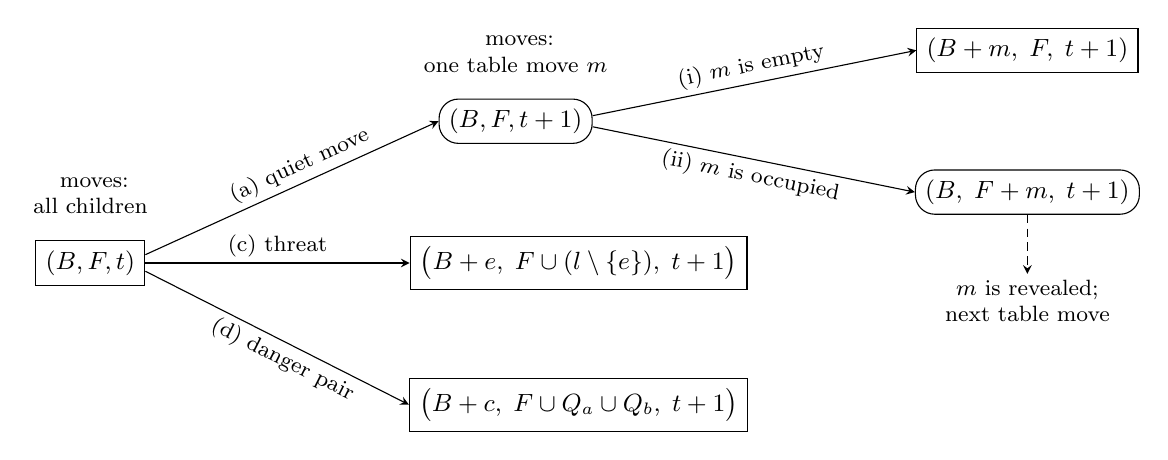
\begin{tikzpicture}[>=stealth,
    pst/.style={draw,rectangle,inner sep=3.5pt,font=\small},
    qst/.style={draw,rectangle,rounded corners=7pt,inner sep=3.5pt,font=\small},
    lbl/.style={font=\footnotesize,inner sep=2pt}]
  \node[pst] (P)  at (0,0)       {$\Pst(B,F,t)$};
  \node[qst] (Q)  at (5.4,1.8)   {$\Qst(B,F,t+1)$};
  \node[pst] (C)  at (6.2,0)     {$\Pst\bigl(B+e,\;F\cup(l\setminus\{e\}),\;t+1\bigr)$};
  \node[pst] (D)  at (6.2,-1.8)  {$\Pst\bigl(B+c,\;F\cup Q_a\cup Q_b,\;t+1\bigr)$};
  \node[pst] (I)  at (11.9,2.7)  {$\Pst(B+m,\;F,\;t+1)$};
  \node[qst] (II) at (11.9,0.9)  {$\Qst(B,\;F+m,\;t+1)$};
  \draw[->] ([yshift=3pt]P.east) -- node[lbl,sloped,above,pos=0.55] {(a) quiet move} (Q.west);
  \draw[->] (P.east) -- node[lbl,above,pos=0.5] {(c) threat} (C.west);
  \draw[->] ([yshift=-3pt]P.east) -- node[lbl,sloped,below,pos=0.55] {(d) danger pair} (D.west);
  \draw[->] ([yshift=2pt]Q.east) -- node[lbl,sloped,above] {(i) $m$ is empty} (I.west);
  \draw[->] ([yshift=-2pt]Q.east) -- node[lbl,sloped,below] {(ii) $m$ is occupied} (II.west);
  \draw[->,densely dashed] (II.south) -- ++(0,-0.75)
        node[lbl,below,align=center] {$m$ is revealed;\\ next table move};
  \node[lbl,align=center] at (0,0.85) {\Maker{} moves:\\ all children};
  \node[lbl,align=center] at (5.4,2.65) {\Breaker{} moves:\\ one table move $m$};
\end{tikzpicture}
\caption{One round of the abstract game. A P-state (\Maker{} to move, sharp corners) has one child \textup{(a)}
and one child \textup{(c)} or \textup{(d)} for every conceivable forced event; all of them must be \WON{} or
\VOID. At a Q-state (\Breaker{} to move, rounded corners) one table move $m$ is chosen; both the case that $m$
is empty and the case that $m$ holds an unrevealed stone of \Maker{} must be covered. Child \textup{(ii)} is
again a Q-state, with one more revealed stone.}
\label{fig:round}
\end{figure}

\cref{fig:round} shows one round. The children are indeed states: in \textup{(c)} we have
$e\notin B$ because $l$ is live and $e\notin F$ by assumption, so $|B+e|=t+1$ and $B+e$ is disjoint from
$F\cup(l\setminus\{e\})$; the same holds in \textup{(d)} for $c$, $Q_a$, $Q_b$; and \textup{(ii)} requires
$|F+m|\le t$. Different data may define the same child.

The meaning is as follows. In \textup{(a)}, the $(t+1)$-th move of \Maker{} has caused no forced event, and the
record does not change except for $t$. In \textup{(c)}, that move has created a threat on $l$ with sixth
cell $e$: \Breaker{} takes $e$, and the five stones on $l$ are revealed. In \textup{(d)}, it has created a
danger pair $\{a,b\}$ with common cell $c$: \Breaker{} takes $c$, and the four stones $Q_a$ on $a$ and the
four stones $Q_b$ on $b$ are revealed. The conditions $F\cap a\subseteq Q_a$, $F\cap b\subseteq Q_b$ say that
the stones already revealed on these lines are among the four, and the bounds by $t+1$ say that \Maker{}
has only $t+1$ stones at this moment. In \textup{(i)} and \textup{(ii)}, the table names the cell $m$ in round
$t$; either $m$ is empty and \Breaker{} takes it, or $m$ holds an unrevealed stone of \Maker, which is thereby
revealed. If $|F|=t$, all stones of \Maker{} are revealed, $m\notin F$ is empty, and no child \textup{(ii)} is
needed.

The lists \textup{(c)} and \textup{(d)} contain every forced event that can occur in a play
(\cref{thm:soundness}), and in general many that cannot: the definition does not ask whether the
stones can be reached by an admissible play. This only makes the requirement \WON{} below stronger. The
letter \textup{(b)} is not used here; it is reserved for an additional kind of child in the eager variant of
\cref{sec:game-remarks}.

The child \textup{(a)} of a non-\VOID{} P-state is not \VOID, and neither is the child \textup{(i)} of a
non-\VOID{} Q-state, because $F$ remains admissible when $m\notin F$ is added to $B$
(\cref{lem:adm-closed}\,(b)). Children \textup{(c)}, \textup{(d)} and \textup{(ii)} can be \VOID.

\subsection{Patterns, the predicate \texorpdfstring{$\LOST$}{LOST}, and winning states}\label{sec:won}

The following two patterns describe the situations in which a forced reply fails to restore admissibility
(\cref{lem:threat,lem:danger}). In both, $x$ plays the role of the stone that \Maker{} has
just placed, and the \emph{stone sets} are the cells that \Maker{} would hold on the lines of the pattern
after this move.

\begin{definition}[Patterns $\Etwo$ and $\Ethree$; $\LOST$]\label{def:lost}
Let $B,F$ be disjoint sets of cells and $t\ge 0$.

An \emph{$\Etwo$ pattern} for $(B,F)$ (a threat and a danger pair) consists of three pairwise distinct live
lines $l,a,b\in\live{B}$, three pairwise distinct cells $x,e,c$, and two sets $S_a,S_b$ of cells such that
\begin{enumerate}[label=\textup{(E2.\arabic*)},leftmargin=3.6em]
\item $l\cap a=\{x\}$, $e\in l$, $a\cap b=\{c\}$, $x\notin b$, $e\notin b$;
\item $S_a\subseteq a\setminus\{c\}$ with $|S_a|=4$ and $x\in S_a$; $S_b\subseteq b\setminus\{c\}$ with $|S_b|=4$;
\item $e\notin F$, $c\notin F$, $F\cap a\subseteq S_a$, $F\cap b\subseteq S_b$.
\end{enumerate}
Its stone sets are $S_l=l\setminus\{e\}$, $S_a$ and $S_b$.

An \emph{$\Ethree$ pattern} for $(B,F)$ (two danger pairs) consists of four pairwise distinct live lines
$a,a',b,b'\in\live{B}$, three pairwise distinct cells $x,c,c'$, and four sets $S_a,S_{a'},S_b,S_{b'}$ of cells
such that
\begin{enumerate}[label=\textup{(E3.\arabic*)},leftmargin=3.6em]
\item $a\cap a'=\{x\}$, $a\cap b=\{c\}$, $a'\cap b'=\{c'\}$, $x\notin b\cup b'$;
\item $S_a\subseteq a\setminus\{c\}$, $S_{a'}\subseteq a'\setminus\{c'\}$, $S_b\subseteq b\setminus\{c\}$,
  $S_{b'}\subseteq b'\setminus\{c'\}$, each of the four sets has exactly four cells, $x\in S_a\cap S_{a'}$,
  and neither $c$ nor $c'$ belongs to any of the four sets;
\item $c\notin F$, $c'\notin F$, $F\cap a\subseteq S_a$, $F\cap a'\subseteq S_{a'}$, $F\cap b\subseteq S_b$,
  $F\cap b'\subseteq S_{b'}$.
\end{enumerate}
Its stone sets are $S_a$, $S_{a'}$, $S_b$ and $S_{b'}$.

A pattern \emph{fits} $(B,F,t)$ if the union of $F$ and all stone sets of the pattern has at most $t+1$ cells.
$\LOST(B,F,t)$ holds if some $\Etwo$ pattern or some $\Ethree$ pattern for $(B,F)$ fits $(B,F,t)$.
\end{definition}

In an $\Etwo$ pattern, $l$ is a threat with sixth cell $e$, and $\{a,b\}$ is a danger pair with common cell
$c$ none of whose lines contains $e$ (note that $e\notin a$, because $e\in l$, $e\ne x$ and
$l\cap a=\{x\}$). In an $\Ethree$ pattern, $\{a,b\}$ and $\{a',b'\}$ are danger pairs with common cells $c$
and $c'$. The condition $e\notin F$ implies $F\cap l\subseteq S_l$.

\begin{definition}[\WON]\label{def:won}
Fix an integer $\Rmax\ge 0$. The label \WON{} (more precisely: \WON{} for $\Rmax$) is defined for states that
are not \VOID, by the following recursion.

A P-state $\Pst(B,F,t)$ that is not \VOID{} is \WON{} if
\begin{enumerate}[label=\textup{(P\arabic*)},leftmargin=3em]
\item $\LEAF(B,F,t)$ holds; or
\item $t<\Rmax$, $\LOST(B,F,t)$ is false, and every child \textup{(a)}, \textup{(c)}, \textup{(d)} of
  $\Pst(B,F,t)$ (\cref{def:states}) is \WON{} or \VOID.
\end{enumerate}
A Q-state $\Qst(B,F,t)$ that is not \VOID{} is \WON{} if there is a cell $m\notin B\cup F$ such that
\begin{enumerate}[label=\textup{(\roman*)},leftmargin=3em]
\item the child \textup{(i)} of $\Qst(B,F,t)$ via $m$ is \WON; and
\item if $|F|<t$, the child \textup{(ii)} of $\Qst(B,F,t)$ via $m$ is \WON{} or \VOID.
\end{enumerate}
Such a cell $m$ is called a \emph{table move} for $\Qst(B,F,t)$.
\end{definition}

In (P1) the predicate $\LEAF(B,F,k)$ of \cref{def:leaf} is used with $k=t\ge|F|$. A P-state with
$t\ge\Rmax$ is \WON{} only if it satisfies (P1). Thus $\Rmax$ bounds the number of rounds that \Breaker{} plays
from the table.

\begin{lemma}[The recursion is well founded]\label{lem:rank}
For states put
\[ \rk\bigl(\Pst(B,F,t)\bigr)=\bigl(2(\Rmax-t),\,0\bigr),\qquad
   \rk\bigl(\Qst(B,F,t)\bigr)=\bigl(2(\Rmax-t)+1,\;t-|F|\bigr), \]
and order these pairs of integers lexicographically. Then every child of a state has smaller rank than the
state itself. Consequently \cref{def:won} defines the label \WON{} uniquely for every state that is
not \VOID.
\end{lemma}

\begin{proof}
The child \textup{(a)} of $\Pst(B,F,t)$ has rank $(2(\Rmax-t)-1,\,\cdot\,)$, and the children \textup{(c)},
\textup{(d)} have rank $(2(\Rmax-t)-2,0)$; all are smaller than $(2(\Rmax-t),0)$ in the first component. The
child \textup{(i)} of $\Qst(B,F,t)$ has rank $(2(\Rmax-t),0)$, which is smaller than
$(2(\Rmax-t)+1,\,t-|F|)$ in the first component, and the child \textup{(ii)} has rank
$(2(\Rmax-t)+1,\,t-|F|-1)$, which is smaller in the second. The condition for a state to be \WON{} refers,
besides the predicates $\LEAF$ and $\LOST$ and the question which children are \VOID, only to the labels of
its children. There are finitely many
states (a state has $t\le|\Q|+1$), so the ranks form a finite totally ordered set, and the label is defined by
recursion on the rank.
\end{proof}

\subsection{Symmetry and certificates}\label{sec:cert}

For $g\in\G$ and a state $\Pst(B,F,t)$ or $\Qst(B,F,t)$, the \emph{image} under $g$ is $\Pst(gB,gF,t)$ or
$\Qst(gB,gF,t)$. The \emph{canonical form} of a state is its image under a map $g\in\G$ for which
$(gB,gF)$ is the canonical form $\canon(B,F)$ of the pair $(B,F)$ (\cref{def:canon}); we
write $\canon\Pst(B,F,t)$ and $\canon\Qst(B,F,t)$. A state is \emph{canonical} if it is its own canonical
form. The root is canonical.

\begin{lemma}[Symmetry of the abstract game]\label{lem:game-invariance}
Let $g\in\G$.
\begin{enumerate}[label=\textup{(\alph*)},leftmargin=2.4em]
\item The image of a state is a state of the same kind, with the same $t$, the same $|F|$ and the same rank.
  A state is \VOID{} if and only if its image is. Moreover $\LEAF(B,F,t)$ holds if and only if
  $\LEAF(gB,gF,t)$ holds, and $\LOST(B,F,t)$ holds if and only if $\LOST(gB,gF,t)$ holds.
\item The children \textup{(a)}, \textup{(c)}, \textup{(d)} of the image of a P-state are exactly the images
  of its children \textup{(a)}, \textup{(c)}, \textup{(d)}. The children \textup{(i)}, \textup{(ii)} of the
  image of a Q-state via $g(m)$ are the images of its children \textup{(i)}, \textup{(ii)} via $m$.
\item A state that is not \VOID{} is \WON{} if and only if its image is \WON; and $m$ is a table move for
  $\Qst(B,F,t)$ if and only if $g(m)$ is a table move for $\Qst(gB,gF,t)$.
\item A state and its image have the same canonical form.
\end{enumerate}
\end{lemma}

\begin{proof}
By \cref{lem:group}, $\G$ is a group of bijections of $\Q$ each of which maps lines onto lines.
(a) and (b): all notions involved are defined in terms of membership of cells in sets, cardinalities, and
the set of lines, and are therefore preserved by a bijection of the cells that permutes the lines. For live
lines, admissibility and $\LEAF$ this is \cref{lem:invariance}\,(a),~(b),~(e). For $\LOST$, the image of a pattern for
$(B,F)$ is a pattern for $(gB,gF)$ with stone sets of the same sizes. For (b), data $(l,e)$ define a
child \textup{(c)} of $\Pst(B,F,t)$ if and only if $(gl,g(e))$ define a child \textup{(c)} of the image, and
the second child is the image of the first; likewise for \textup{(a)}, \textup{(d)}, \textup{(i)},
\textup{(ii)}. Applying this to $g^{-1}$ shows that every child of the image arises in this way.
(c) follows from (a) and (b) by induction on the rank. (d) is \cref{lem:canon}\,(a).
\end{proof}

\begin{definition}[Certificate]\label{def:certificate}
A \emph{certificate} is a triple $(\Tbl,\Lv,\Rmax)$, where $\Rmax\ge 0$ is an integer, $\Lv$ is a finite set
of canonical P-states (the \emph{leaves}), and $\Tbl$ (the \emph{table}) is a map from a finite set of
canonical Q-states to cells. The \emph{reachable set} $V$ of the certificate is the smallest set of
canonical states such that
\begin{enumerate}[label=\textup{(R\arabic*)},leftmargin=3em,start=0]
\item the root $\Pst(\emptyset,\emptyset,0)$ belongs to $V$;
\item if a P-state $P\in V$ is not in $\Lv$, then the canonical form of every child \textup{(a)},
  \textup{(c)}, \textup{(d)} of $P$ that is not \VOID{} belongs to $V$;
\item if $Q=\Qst(B,F,t)\in V$, and $m=\Tbl(Q)$ is defined and $m\notin B\cup F$, then the canonical form of the
  child \textup{(i)} of $Q$ via $m$ belongs to $V$, and so does the canonical form of the child \textup{(ii)}
  of $Q$ via $m$ if this child exists and is not \VOID.
\end{enumerate}
The certificate is \emph{valid} if
\begin{enumerate}[label=\textup{(V\arabic*)},leftmargin=3em]
\item $\LEAF(B,F,t)$ holds for every $\Pst(B,F,t)\in V\cap\Lv$;
\item every $\Pst(B,F,t)\in V\setminus\Lv$ satisfies $t<\Rmax$, and $\LOST(B,F,t)$ is false;
\item for every $\Qst(B,F,t)\in V$, the cell $\Tbl\bigl(\Qst(B,F,t)\bigr)$ is defined and does not belong to
  $B\cup F$.
\end{enumerate}
\end{definition}

The reachable set is finite and is obtained by a search from the root; checking (V1)--(V3) along this search
is what a verifier of a certificate does (\cref{alg:verify}). Leaves and table entries outside $V$
are irrelevant.

\begin{lemma}[Certificates and \WON]\label{lem:certificate}
Let $(\Tbl,\Lv,\Rmax)$ be a certificate with reachable set $V$.
\begin{enumerate}[label=\textup{(\alph*)},leftmargin=2.4em]
\item No state of $V$ is \VOID.
\item If the certificate is valid, then every state of $V$ is \WON{} for $\Rmax$. In particular the root is
  \WON.
\item Conversely, if the root is \WON{} for $\Rmax$, then there is a valid certificate with this $\Rmax$.
\end{enumerate}
\end{lemma}

\begin{proof}
(a) The set of all canonical states that are not \VOID{} satisfies (R0)--(R2): the root is not \VOID; the
child \textup{(i)} of a Q-state that is not \VOID{} is not \VOID; all other children enter $V$ only if they
are not \VOID; and the canonical form of a state that is not \VOID{} is not \VOID{}
(\cref{lem:game-invariance}\,(a)). Since $V$ is the smallest set with (R0)--(R2), it is contained in this
set.

(b) We show by induction on the rank that every $S\in V$ is \WON. Recall that a state and its canonical form
have the same rank, and that one is \WON{} if and only if the other is (\cref{lem:game-invariance}).
If $S=\Pst(B,F,t)\in\Lv$, then $S$ satisfies (P1) by (V1). If $S=\Pst(B,F,t)\notin\Lv$, then $t<\Rmax$ and
$\LOST(B,F,t)$ is false by (V2). The canonical form of every child of $S$ that is not \VOID{} belongs to $V$
by (R1) and has smaller rank than $S$, so it is \WON{} by induction, and hence so is the child. Thus $S$
satisfies (P2). If $S=\Qst(B,F,t)$, then $m=\Tbl(S)$ is defined and $m\notin B\cup F$ by (V3). By (R2) and by
induction the child \textup{(i)} of $S$ via $m$ is \WON, and the child \textup{(ii)}, if it exists, is \VOID{}
or \WON. So $m$ is a table move for $S$, and $S$ is \WON.

(c) Let $\Lv$ be the set of all canonical P-states $\Pst(B,F,t)$ for which $\LEAF(B,F,t)$ holds, and for every
canonical Q-state that is not \VOID{} and is \WON{} choose a table move as the value of $\Tbl$. Let $W$ be
the set of all canonical states that are not \VOID{} and are \WON. We claim that $W$ satisfies (R0)--(R2),
so that $V\subseteq W$. The root belongs to $W$ by assumption. Let $P=\Pst(B,F,t)\in W\setminus\Lv$. Then
(P1) fails, so (P2) holds: every child of $P$ is \WON{} or \VOID, and the canonical form of a child that is
not \VOID{} is in $W$. Let $Q=\Qst(B,F,t)\in W$. Then $m=\Tbl(Q)$ is a table move, so $m\notin B\cup F$, the
child \textup{(i)} via $m$ is \WON, and the child \textup{(ii)}, if it exists and is not \VOID, is \WON; their
canonical forms are in $W$. This proves the claim. Now (V1) holds by the choice of $\Lv$. A P-state in
$V\setminus\Lv$ is \WON{} and violates (P1), so it satisfies (P2), which contains (V2). A Q-state in $V$ is a
canonical \WON{} state, so the table is defined there and its value is a table move, which gives (V3).
\end{proof}

\subsection{The strategy \texorpdfstring{$\sigma$}{sigma}}\label{sec:sigma}

\begin{definition}[The strategy $\sigma$]\label{def:sigma}
Let $(\Tbl,\Lv,\Rmax)$ be a certificate. \Breaker{} keeps a record $(B,F,t)$ and a \emph{mode}, which is
\TABLE{} or \PAIRING. Initially $B=F=\emptyset$, $t=0$, and the mode is \TABLE. Let $X$ always denote the set
of stones of \Maker{} on the board. Round $t+1$ (for $t=0,1,2,\dots$) runs as follows.
\begin{enumerate}[label=\textup{(S\arabic*)},leftmargin=3em]
\item\label{S:leaf} \emph{Leaf test.} If the mode is \TABLE{} and $\canon\Pst(B,F,t)\in\Lv$, then
  \Breaker{} computes a pairing $\pi$ for $(B,X)$ and switches to \PAIRING{} mode for the rest of the game.
\item\label{S:maker} \emph{Move of \Maker.} \Maker{} occupies an empty cell $x$. Put $X'=X+x$.
\item\label{S:pairing} \emph{Reply in \PAIRING{} mode.} If $x\in\pi(l)$ for a line $l\in\live{B}$ and the
  other cell of $\pi(l)$ is empty, \Breaker{} takes this other cell. Otherwise \Breaker{} takes an
  arbitrary empty cell, say the empty cell $(x_1,x_2,x_3)$ with the smallest id $36x_1+6x_2+x_3$.
\end{enumerate}
In \TABLE{} mode \Breaker{} applies the first of the following three rules that is applicable.
\begin{enumerate}[label=\textup{(S\arabic*)},leftmargin=3em,start=4]
\item\label{S:threat} \emph{Threat rule.} If some line $l\in\live{B}$ has five cells in $X'$, let $e$ be the
  sixth cell of $l$. \Breaker{} takes $e$. The new record is
  $\bigl(B+e,\;F\cup(l\setminus\{e\}),\;t+1\bigr)$.
\item\label{S:danger} \emph{Danger rule.} If $X'$ has a danger pair with respect to $B$, let $\{a,b\}$ be the
  danger pair whose common cell $c$ has the smallest id. \Breaker{} takes $c$. The new record is
  $\bigl(B+c,\;F\cup(X'\cap a)\cup(X'\cap b),\;t+1\bigr)$.
\item\label{S:table} \emph{Table rule.} Choose $g\in\G$ with $(gB,gF)=\canon(B,F)$, and put
  \[ m^{\mathrm c}=\Tbl\bigl(\Qst(gB,gF,t+1)\bigr),\qquad m=g^{-1}(m^{\mathrm c}). \]
  \begin{itemize}[leftmargin=1.5em]
  \item If $m\in X'$, replace $F$ by $F+m$ and apply \ref{S:table} again.
  \item If $m\notin X'$, \Breaker{} takes $m$. The new record is $(B+m,\;F,\;t+1)$.
  \end{itemize}
\end{enumerate}
The strategy is \emph{undefined} at a position if no pairing for $(B,X)$ exists in \ref{S:leaf}, if the table
has no entry for the Q-state in \ref{S:table}, or if the cell to be taken is not empty.
\end{definition}

Some comments are in order. In \PAIRING{} mode the record is no longer changed, and in \ref{S:pairing} the
set $B$ and the pairing $\pi$ are those of the moment of the switch. The pairs $\pi(l)$ are pairwise
disjoint, so the line $l$ in \ref{S:pairing} is unique; the proviso ``is empty'' is necessary, because the
other cell of $\pi(l)$ may already hold a stone that \Breaker{} placed earlier as an arbitrary move. In \ref{S:threat} the line $l$ is unique in all positions that matter
(\cref{lem:one-move}\,(a)); for definiteness take the first such line in a fixed order. In
\ref{S:danger} the danger pair is determined by its common cell (\cref{lem:one-move}\,(d)). In
\ref{S:table} the map $g$ need not be unique; any $g\in\G$ that attains the canonical form may be used
(\cref{lem:canon}\,(b),~(c)), and for definiteness the first one in a fixed enumeration of $\G$ is taken. With these conventions $\sigma$
prescribes at most one cell in every position, as a function of the moves played so far. The record is
changed only at the end of the round, except that \ref{S:table} may enlarge $F$ several times before a move
is found: every repetition reveals one more stone of \Maker.

\cref{thm:soundness} below shows that for a valid certificate $\sigma$ is never undefined. A pairing in
\ref{S:leaf} can be computed by a maximum flow (\cref{lem:hall}\,(c)).

\subsection{The number of stones of a pattern}\label{sec:stones}

\begin{proposition}[Stones of a pattern]\label{prop:lost-stones}
Let $B,F$ be disjoint sets of cells.
\begin{enumerate}[label=\textup{(\alph*)},leftmargin=2.4em]
\item For every $\Etwo$ pattern for $(B,F)$,
  $|S_l\cup S_a\cup S_b| = 12-|S_l\cap S_b|$ and $|S_l\cap S_b|\le 1$. Hence the stone sets of an
  $\Etwo$ pattern contain at least $11$ distinct cells.
\item For every $\Ethree$ pattern for $(B,F)$,
  \[ |S_a\cup S_{a'}\cup S_b\cup S_{b'}| \;=\; 15-|S_a\cap S_{b'}|-|S_{a'}\cap S_b|-|S_b\cap S_{b'}|, \]
  and each of the three intersections has at most one cell. Hence the stone sets of an $\Ethree$ pattern
  contain at least $12$ distinct cells.
\item $\LOST(B,F,t)$ is false whenever $t\le 9$. Consequently, in a certificate with $\Rmax\le 10$ the
  requirement ``$\LOST(B,F,t)$ is false'' of \textup{(V2)}, and of \textup{(P2)}, is satisfied automatically.
\end{enumerate}
\end{proposition}

\begin{proof}
The lines of a pattern are pairwise distinct, so any two of them have at most one common cell
(\cref{lem:geometry}).

(a) We have $|S_l|=5$ and $|S_a|=|S_b|=4$. First, $S_l\cap S_a=\{x\}$: the intersection is contained in
$l\cap a=\{x\}$, and $x$ belongs to $S_a$ by (E2.2) and to $S_l=l\setminus\{e\}$ because $x\in l$
and $x\ne e$. Second, $S_a\cap S_b=\emptyset$: the intersection is contained in $a\cap b=\{c\}$, and
$c\notin S_a$. Third, $S_l\cap S_b\subseteq l\cap b$ has at most one cell. The intersection of all three
sets is contained in $S_a\cap S_b=\emptyset$. By inclusion--exclusion,
$|S_l\cup S_a\cup S_b|=(5+4+4)-(1+0+|S_l\cap S_b|)+0$.

(b) Each of the four stone sets has four cells. Of the six pairwise intersections, $S_a\cap S_{a'}=\{x\}$,
because it is contained in $a\cap a'=\{x\}$ and $x\in S_a\cap S_{a'}$ by (E3.2); $S_a\cap S_b=\emptyset$,
because it is contained in $a\cap b=\{c\}$ and $c$ is in no stone set; and $S_{a'}\cap S_{b'}=\emptyset$ for the
same reason with $c'$. The remaining three, $S_a\cap S_{b'}$, $S_{a'}\cap S_b$ and $S_b\cap S_{b'}$, are
contained in the intersection of two distinct lines and have at most one cell each. Any three of the four
stone sets include both $S_a$ and $S_b$, or both $S_{a'}$ and $S_{b'}$; hence all intersections of three or
four of the stone sets are empty. By inclusion--exclusion the union has
$16-\bigl(1+0+0+|S_a\cap S_{b'}|+|S_{a'}\cap S_b|+|S_b\cap S_{b'}|\bigr)$ cells.

(c) If a pattern fits $(B,F,t)$, then the union of $F$ and its stone sets has at most $t+1$ cells; by (a)
and (b) this union has at least $11$ cells. So $\LOST(B,F,t)$ implies $t\ge 10$. A state
$\Pst(B,F,t)\in V\setminus\Lv$ of a certificate with $\Rmax\le 10$ that satisfies the first half of (V2) has
$t\le 9$.
\end{proof}

The bounds $11$ and $12$ are all that is needed. On the $6\times6\times6$ board the value $11$ is attained
for $\Etwo$, whereas an $\Ethree$ pattern has in fact at least $13$ distinct stones
(\cref{sec:extra-e23}). The same counting gives a cheap necessary condition, which lets an
implementation reject most states without searching for patterns: the stone sets of an $\Etwo$ pattern
contain $5-|F\cap l|$, $4-|F\cap a|$ and $4-|F\cap b|$ cells outside $F$, of which at most two coincide, so
that a fitting $\Etwo$ pattern has
$(5-|F\cap l|)+(4-|F\cap a|)+(4-|F\cap b|)-2\le t+1-|F|$.

\subsection{One move of \texorpdfstring{\Maker}{Maker} from an admissible position}\label{sec:one-move}

The next three lemmas analyze what a single move of \Maker{} can do to an admissible position. They are the
link between real plays and the children \textup{(c)}, \textup{(d)} and the patterns $\Etwo$, $\Ethree$.

\begin{lemma}[One move]\label{lem:one-move}
Let $X$ be $B$-admissible, let $x\notin B\cup X$ be a cell, and let $X'=X+x$. Threats and danger pairs refer
to $B$.
\begin{enumerate}[label=\textup{(\alph*)},leftmargin=2.4em]
\item No live line has six cells in $X'$. At most one live line has five cells in $X'$; such a line contains
  $x$.
\item In every danger pair of $X'$ exactly one of the two lines contains $x$. This line, the \emph{new line}
  of the pair, has exactly three cells in $X$. The other line, the \emph{old line} of the pair, has exactly
  four cells in $X$. The common cell $c$ of the pair is different from $x$ and is empty, that is,
  $c\notin B\cup X'$.
\item Two distinct old lines of danger pairs of $X'$ have no common cell outside $X'$. Two distinct new
  lines of danger pairs of $X'$ have exactly the cell $x$ in common.
\item Distinct danger pairs of $X'$ have distinct common cells.
\end{enumerate}
\end{lemma}

\noindent In the sequel a danger pair of $X'$ is written as an ordered pair $(a,b)$, with $a$ its new line and
$b$ its old line.

\begin{proof}
(a) A live line has at most four cells in $X$, hence at most five in $X'$, and exactly five only if it
contains $x$ and has exactly four cells in $X$. Two distinct live lines of this kind would share the cell
$x\notin X$ and would form a danger pair of $X$, which does not exist.

(b) Let $\{a,b\}$ be a danger pair of $X'$ with common cell $c\notin X'$. If neither line contained $x$,
then $a\cap X=a\cap X'$ and $b\cap X=b\cap X'$ would have four cells each, and $c\notin X$: a danger pair of
$X$. If both lines contained $x$, then $a\cap b=\{x\}$ by \cref{lem:geometry}, so $c=x\in X'$, which is
false. So exactly one line contains $x$; it has $4-1=3$ cells in $X$, and the other line has four cells in
$X$. Finally $c\ne x$ because $c\notin X'$, and $c\notin B$ because the lines are live.

(c) An old line has exactly four cells in $X$ by (b). If two distinct old lines had a common cell outside
$X'\supseteq X$, they would form a danger pair of $X$. Two distinct new lines both contain $x$, and they have
no other common cell by \cref{lem:geometry}.

(d) Let $(a,b)$ and $(a',b')$ be danger pairs of $X'$ with the same common cell $c$. The new lines $a$ and
$a'$ both contain the two distinct cells $x$ and $c$, so $a=a'$ by \cref{lem:geometry}. The old lines $b$
and $b'$ both contain $c\notin X'$, so $b=b'$ by (c).
\end{proof}

\begin{lemma}[Threat]\label{lem:threat}
Let $X$ be $B$-admissible, $F\subseteq X$ and $t=|X|$. Let $x\notin B\cup X$ and $X'=X+x$. Suppose that a live
line $l\in\live{B}$ has five cells in $X'$, and let $e$ be its sixth cell. Then $e$ is empty, and one of the
following holds:
\begin{enumerate}[label=\textup{(\arabic*)},leftmargin=2.4em]
\item $X'$ is $(B+e)$-admissible; or
\item some $\Etwo$ pattern for $(B,F)$ fits $(B,F,t)$, so that $\LOST(B,F,t)$ holds.
\end{enumerate}
\end{lemma}

\begin{proof}
We have $e\notin X'$ by the choice of $e$, and $e\notin B$ because $l$ is live. Hence $e$ is empty and
$X'\cap(B+e)=\emptyset$. The lines that are live with respect to $B+e$ are the lines of $\live{B}$ that do
not contain $e$. By \cref{lem:one-move}\,(a), $l$ is the only line of $\live{B}$ with more than four
cells in $X'$, and $l$ contains $e$. So every line that is live with respect to $B+e$ has at most four
cells in $X'$.

Suppose that (1) fails. Then $X'$ has a danger pair with respect to $B+e$. This is a danger pair $(a,b)$ of
$X'$ with respect to $B$ such that $e\notin a\cup b$; let $a$ be its new line, $b$ its old line and $c$ its
common cell (\cref{lem:one-move}\,(b)). We verify that the lines $l,a,b$, the cells $x,e,c$ and the sets
$S_a=X'\cap a$, $S_b=X'\cap b$ form an $\Etwo$ pattern for $(B,F)$. The three lines are live with respect to
$B$. They are pairwise distinct: $a\ne b$, and $e$ lies on $l$ but not on $a$ or $b$. The three cells are
pairwise distinct: $x\in X'$ whereas $e,c\notin X'$, and $c\in a$ whereas $e\notin a$.
\begin{itemize}[leftmargin=2.2em]
\item (E2.1): $x\in l$ by \cref{lem:one-move}\,(a) and $x\in a$, so $l\cap a=\{x\}$ by
  \cref{lem:geometry}; $e\in l$; $a\cap b=\{c\}$ by \cref{lem:geometry}; $x\notin b$ because $b$ is
  the old line; $e\notin b$.
\item (E2.2): $S_a$ and $S_b$ have four cells each because $(a,b)$ is a danger pair of $X'$; they do not
  contain $c$ because $c\notin X'$; and $x\in S_a$.
\item (E2.3): $F\subseteq X\subseteq X'$, hence $e\notin F$, $c\notin F$, $F\cap a\subseteq X'\cap a=S_a$
  and $F\cap b\subseteq S_b$.
\end{itemize}
The stone sets are $S_l=l\setminus\{e\}=X'\cap l$, $S_a$ and $S_b$. Their union with $F$ is contained
in $X'$ and therefore has at most $|X'|=t+1$ cells: the pattern fits $(B,F,t)$.
\end{proof}

\begin{lemma}[Danger]\label{lem:danger}
Let $X$ be $B$-admissible, $F\subseteq X$ and $t=|X|$. Let $x\notin B\cup X$ and $X'=X+x$. Suppose that no live
line has five cells in $X'$ and that $X'$ has at least one danger pair with respect to $B$. Let $(a,b)$ be
\emph{any} danger pair of $X'$, and let $c$ be its common cell. Then $c$ is empty, and one of the following
holds:
\begin{enumerate}[label=\textup{(\arabic*)},leftmargin=2.4em]
\item $X'$ is $(B+c)$-admissible; or
\item some $\Ethree$ pattern for $(B,F)$ fits $(B,F,t)$, so that $\LOST(B,F,t)$ holds.
\end{enumerate}
More precisely, if no $\Ethree$ pattern fits $(B,F,t)$, then any two danger pairs of $X'$ have a line in
common, and either all danger pairs of $X'$ have the same new line or all of them have the same old line.
\end{lemma}

\begin{proof}
The cell $c$ is empty by \cref{lem:one-move}\,(b), so $X'\cap(B+c)=\emptyset$. By
\cref{lem:one-move}\,(a) and the hypothesis, every line of $\live{B}$ has at most four cells in $X'$. The
lines that are live with respect to $B+c$ are the lines of $\live{B}$ that do not contain $c$. Therefore
$X'$ is $(B+c)$-admissible unless there is a danger pair of $X'$ with respect to $B$ none of whose lines
contains $c$.

Let $(a',b')$ be a danger pair of $X'$ with respect to $B$ such that $a'\ne a$ and $b'\ne b$, and let $c'$ be
its common cell. We verify that the lines $a,a',b,b'$, the cells $x,c,c'$ and the sets $S_a=X'\cap a$,
$S_{a'}=X'\cap a'$, $S_b=X'\cap b$, $S_{b'}=X'\cap b'$ form an $\Ethree$ pattern for $(B,F)$. The four lines are
live with respect to $B$. They are pairwise distinct: $a\ne a'$ and $b\ne b'$ by assumption, and the new
lines $a,a'$ contain $x$ while the old lines $b,b'$ do not. The three cells are pairwise distinct: $x\in X'$
whereas $c,c'\notin X'$, and $c\ne c'$ by \cref{lem:one-move}\,(d).
\begin{itemize}[leftmargin=2.2em]
\item (E3.1): $a\cap a'=\{x\}$ by \cref{lem:one-move}\,(c); $a\cap b=\{c\}$ and $a'\cap b'=\{c'\}$ by
  \cref{lem:geometry}; $x\notin b\cup b'$ because $b$ and $b'$ are old lines.
\item (E3.2): each of the four sets has four cells because the lines belong to danger pairs of $X'$; the
  sets do not contain $c$ or $c'$ because $c,c'\notin X'$, and in particular they are contained in
  $a\setminus\{c\}$, $a'\setminus\{c'\}$, $b\setminus\{c\}$, $b'\setminus\{c'\}$, respectively; and
  $x\in S_a\cap S_{a'}$.
\item (E3.3): $F\subseteq X\subseteq X'$, hence $c,c'\notin F$ and $F\cap a\subseteq X'\cap a=S_a$, and
  likewise for $a'$, $b$, $b'$.
\end{itemize}
The union of $F$ and the four stone sets is contained in $X'$ and has at most $t+1$ cells: the pattern fits
$(B,F,t)$.

Now suppose that no $\Ethree$ pattern fits $(B,F,t)$. By what was just shown, every danger pair $(a',b')$ of
$X'$ has $a'=a$ or $b'=b$, so one of its lines contains $c\in a\cap b$. Hence no danger pair of $X'$ with
respect to $B$ avoids $c$, and (1) holds. Since $(a,b)$ was arbitrary, any two danger pairs have a line in
common: the new line or the old line, and not both if the pairs are different. If two different pairs have
the same new line $a_1$, so that their old lines $b_1\ne b_2$ differ, then a pair with a new line different
from $a_1$ would have to have the old line $b_1$ and the old line $b_2$, which is impossible; so all pairs
have the new line $a_1$. Otherwise no two different pairs have the same new line, and then any two pairs
have the same old line.
\end{proof}

\begin{remark}[At most one forced event with ten stones]\label{rem:one-event}
In the situation of \cref{lem:one-move} suppose that $|X'|\le 10$. Then $X'$ has no threat and no danger
pair, or exactly one threat and no danger pair, or no threat and exactly one danger pair. Indeed, there is
at most one threat by \cref{lem:one-move}\,(a). A threat $l$ together with a danger pair $(a,b)$
requires at least $5+4+4-2=11$ stones, since $l\cap a=\{x\}$ (both lines contain $x$, and they are
distinct because they have different numbers of cells in $X'$), the common cell of $a$ and $b$ is not in
$X'$, and $l$ and $b$ share at most one cell. Two danger pairs with the same new line $a$ and old lines
$b\ne b'$ require at least $4+4+4-1=11$ stones, since the cells $a\cap b$ and $a\cap b'$ are not in $X'$ and
$b$, $b'$ share at most one cell. Two danger pairs with new lines $a\ne a'$ and the same old line $b$ require
$(4+4-1)+4=11$ stones, since $a\cap a'=\{x\}$ and the cells $a\cap b$, $a'\cap b$ are not in $X'$. Two danger
pairs with different new lines and different old lines require at least $12$ stones by the proof of
\cref{lem:danger} and \cref{prop:lost-stones}\,(b). Consequently, when \Breaker{} follows $\sigma$ for a valid certificate with $\Rmax\le 10$, the forced reply
in \TABLE{} mode is always unique and the choice in rule \ref{S:danger} is never exercised: there $X$ is
$B$-admissible and $|X'|=t+1\le\Rmax$ by \cref{thm:soundness} below.
\end{remark}

\subsection{Soundness}\label{sec:soundness}

\begin{theorem}[Soundness of the abstract game]\label{thm:soundness}
Let $(\Tbl,\Lv,\Rmax)$ be a valid certificate with reachable set $V$, and let \Breaker{} play the strategy
$\sigma$ of \cref{def:sigma} against arbitrary moves of \Maker. Consider a round that begins in
\TABLE{} mode. Let $t$ be the number of completed rounds, $X$ the set of stones of \Maker, and $(B,F,t)$ the
record of \Breaker{} at the beginning of this round. Then:
\begin{enumerate}[label=\textup{(I\arabic*)},leftmargin=3em]
\item\label{I:V} $\canon\Pst(B,F,t)\in V$; in particular $\Pst(B,F,t)$ is not \VOID{} and is \WON;
\item\label{I:B} $B$ is exactly the set of stones of \Breaker, and $|B|=t$;
\item\label{I:F} $F\subseteq X$ and $|X|=t$;
\item\label{I:adm} $X$ is $B$-admissible.
\end{enumerate}
Moreover, in this round $\sigma$ is defined: if $\canon\Pst(B,F,t)\in\Lv$, then a pairing for $(B,X)$ exists;
otherwise $t<\Rmax$, and after the move of \Maker{} the rules \ref{S:threat}--\ref{S:table} yield a cell that
is empty, where every look-up in rule \ref{S:table} finds a table entry and rule \ref{S:table} is repeated
at most $t+1-|F|$ times.
\end{theorem}

\begin{proof}
We use induction on $t$. For $t=0$ we have $B=F=X=\emptyset$, the root belongs to $V$, and
\ref{I:V}--\ref{I:adm} hold. Now consider a round that begins in \TABLE{} mode and for which
\ref{I:V}--\ref{I:adm} hold. We show that $\sigma$ is defined in this round, and that
\ref{I:V}--\ref{I:adm} hold at the beginning of the next round unless $\sigma$ has switched to \PAIRING{} mode.
Choose $g\in\G$ with $(gB,gF)=\canon(B,F)$, and let $P^{\mathrm c}=\Pst(gB,gF,t)$, which belongs to $V$
by \ref{I:V}. That $\Pst(B,F,t)$ is not \VOID{} and is \WON{} follows from
\cref{lem:certificate}\,(a),~(b) and \cref{lem:game-invariance}.

\smallskip\noindent\emph{Leaf.} Suppose $P^{\mathrm c}\in\Lv$. By (V1), $\LEAF(gB,gF,t)$ holds, hence
$\LEAF(B,F,t)$ holds (\cref{lem:game-invariance}\,(a)), and hence $\CC(B,F,t)$ holds
(\cref{thm:leaf-implies-C}): every $B$-admissible set that contains $F$ and has at most $t$ cells has
a pairing. By \ref{I:F} and \ref{I:adm}, $X$ is such a set. So a pairing for $(B,X)$ exists, rule
\ref{S:leaf} is defined, and $\sigma$ switches to \PAIRING{} mode. Nothing more is claimed in this case; from
here on the pairing strategy of \cref{lem:pairing} takes over (see the proof of
\cref{thm:sigma}).

\smallskip\noindent\emph{Expanded state.} Suppose $P^{\mathrm c}\notin\Lv$. By (V2) and
\cref{lem:game-invariance}\,(a), $t<\Rmax$ and
\begin{equation}\label{eq:notlost}
  \LOST(B,F,t)\ \text{is false.}
\end{equation}
By (R1), the canonical form of every child \textup{(a)}, \textup{(c)}, \textup{(d)} of $P^{\mathrm c}$ that is
not \VOID{} belongs to $V$. By \cref{lem:game-invariance}\,(a),~(b),~(d) these canonical forms are exactly the
canonical forms of the children of $\Pst(B,F,t)$ that are not \VOID. Thus
\begin{equation}\label{eq:children}
  \begin{minipage}{0.84\textwidth}\centering
  the canonical form of every child \textup{(a)}, \textup{(c)}, \textup{(d)} of $\Pst(B,F,t)$\\
  that is not \VOID{} belongs to $V$.
  \end{minipage}
\end{equation}
If the board is full, the game is over. Otherwise \Maker{} occupies an empty cell $x$. Let $X'=X+x$; then $|X'|=t+1$ and $x\notin B\cup X$ by \ref{I:B}, so
\crefrange{lem:one-move}{lem:danger} apply to $B$, $X$, $F$, $t$ and $x$. Exactly one of the following
three cases occurs, and $\sigma$ distinguishes them by the rules \ref{S:threat}, \ref{S:danger},
\ref{S:table}.

\smallskip\noindent\emph{Case 1: some live line has five cells in $X'$.} By \cref{lem:one-move}\,(a) this
line $l$ is unique. Rule \ref{S:threat} prescribes its sixth cell $e$, which is empty by
\cref{lem:threat}. The new record is $(B',F',t+1)$ with $B'=B+e$ and $F'=F\cup(l\setminus\{e\})$. By
\eqref{eq:notlost} and \cref{lem:threat}, $X'$ is $B'$-admissible. The state $\Pst(B',F',t+1)$ is a child
\textup{(c)} of $\Pst(B,F,t)$, defined by $l$ and $e$: the line $l$ is live; $e\in l\setminus F$
because $e\notin X'\supseteq F$; and $F\cup(l\setminus\{e\})\subseteq X'$, since
$l\setminus\{e\}=X'\cap l$, so this set has at most $t+1$ cells. This child is not \VOID, because
$F'\subseteq X'$ and $X'$ is $B'$-admissible (\cref{lem:adm-closed}\,(a)). By \eqref{eq:children} its
canonical form belongs to $V$. Hence \ref{I:V}--\ref{I:adm} hold at the beginning of the next round, with
$(B',F',t+1)$ and $X'$.

\smallskip\noindent\emph{Case 2: no live line has five cells in $X'$, and $X'$ has a danger pair.} Rule
\ref{S:danger} selects a danger pair $(a,b)$ with common cell $c$ and prescribes $c$, which is empty by
\cref{lem:danger}. The new record is $(B',F',t+1)$ with $B'=B+c$ and
$F'=F\cup(X'\cap a)\cup(X'\cap b)$. By \eqref{eq:notlost} and \cref{lem:danger}, $X'$ is $B'$-admissible.
The state $\Pst(B',F',t+1)$ is a child \textup{(d)} of $\Pst(B,F,t)$, defined by $a$, $b$, $Q_a=X'\cap a$ and
$Q_b=X'\cap b$: the lines $a\ne b$ are live and $a\cap b=\{c\}$; $c\notin F$ and $c\notin Q_a\cup Q_b$ because
$c\notin X'\supseteq F$; $|Q_a|=|Q_b|=4$ by the definition of a danger pair; $F\cap a\subseteq Q_a$ and
$F\cap b\subseteq Q_b$ because $F\subseteq X'$; and $F\cup Q_a\cup Q_b\subseteq X'$ has at most $t+1$ cells.
This child is not \VOID, because $F'\subseteq X'$ and $X'$ is $B'$-admissible. By \eqref{eq:children} its
canonical form belongs to $V$, and \ref{I:V}--\ref{I:adm} hold at the beginning of the next round.

\smallskip\noindent\emph{Case 3: no live line has five cells in $X'$, and $X'$ has no danger pair.} Then $X'$
is $B$-admissible: it is disjoint from $B$, no live line has more than four cells in $X'$
(\cref{lem:one-move}\,(a)), and there is no danger pair. Now $\sigma$ applies rule \ref{S:table}, possibly
several times. We claim that each time rule \ref{S:table} is entered, the current set $F$ satisfies
\begin{equation}\label{eq:loop}
  \canon\Qst(B,F,t+1)\in V\qquad\text{and}\qquad F\subseteq X'.
\end{equation}
At the first entry, $F\subseteq X\subseteq X'$, and $\Qst(B,F,t+1)$ is the child \textup{(a)} of
$\Pst(B,F,t)$, which is not \VOID; so \eqref{eq:loop} holds by \eqref{eq:children}. Suppose \eqref{eq:loop}
holds at some entry. Let $g'\in\G$ be the map chosen by the rule, so that
$Q^{\mathrm c}=\Qst(g'B,g'F,t+1)$ is the canonical form of $\Qst(B,F,t+1)$ and belongs to $V$. By (V3) the
table entry $m^{\mathrm c}=\Tbl(Q^{\mathrm c})$ exists and $m^{\mathrm c}\notin g'B\cup g'F$; hence
$m=g'^{-1}(m^{\mathrm c})\notin B\cup F$. By (R2) and \cref{lem:game-invariance}\,(b),~(d), the canonical
form of the child \textup{(i)} of $\Qst(B,F,t+1)$ via $m$ belongs to $V$, and so does the canonical form of
its child \textup{(ii)} via $m$ if this child exists and is not \VOID.
\begin{itemize}[leftmargin=2.2em]
\item If $m\in X'$, then $m\in X'\setminus F$, so $|F|<|X'|=t+1$ and the child \textup{(ii)},
  $\Qst(B,F+m,t+1)$, exists. It is not \VOID, because $F+m\subseteq X'$ and $X'$ is $B$-admissible
  (\cref{lem:adm-closed}\,(a)). So \eqref{eq:loop} holds for $F+m$, with which the rule is entered again.
  Every such step moves a cell of $X'\setminus F$ into $F$, so there are at most $|X'\setminus F|$ of them,
  counted from the first entry; this number is $t+1-|F|$ for the set $F$ at the beginning of the round.
\item If $m\notin X'$, then $m$ is empty, because $m\notin B$ and $B$ is the set of all stones of \Breaker{}
  by \ref{I:B}. \Breaker{} takes $m$, and the new record is $(B+m,F,t+1)$, where $F$ is the current set. The
  canonical form of the child \textup{(i)}, $\Pst(B+m,F,t+1)$, belongs to $V$; this is \ref{I:V}. Clearly
  \ref{I:B} holds; \ref{I:F} holds by \eqref{eq:loop} and $|X'|=t+1$; and $X'$ is $(B+m)$-admissible because
  it is $B$-admissible and $m\notin X'$ (\cref{lem:adm-closed}\,(b)), which is \ref{I:adm}.
\end{itemize}
In all three cases $\sigma$ was defined, the cell prescribed was empty, and \ref{I:V}--\ref{I:adm} hold at the
beginning of the next round.
\end{proof}

Three features of the proof deserve to be pointed out. All cardinality conditions in the definitions of the
children \textup{(c)}, \textup{(d)}, \textup{(ii)} and of the patterns were verified in the same way: the
sets in question are subsets of $X'$, and $|X'|=t+1$. A \VOID{} child is never entered, since the revealed set
is always a subset of the real set $X'$ of stones of \Maker, which is admissible with respect to the new set
of stones of \Breaker. And the proof does not use any property of the cells named by the table, nor the
particular choice of the danger pair in rule \ref{S:danger}, nor the choice of $g$ in rule \ref{S:table}.

\subsection{Proof of \texorpdfstring{\cref{thm:main}}{the main theorem}}\label{thm:main-proof}

We first state precisely what the strategy $\sigma$ achieves.

\begin{theorem}[The strategy $\sigma$]\label{thm:sigma}
Let $(\Tbl,\Lv,\Rmax)$ be a valid certificate, and let \Breaker, moving second, play the strategy $\sigma$ of
\cref{def:sigma}. Then, whatever \Maker{} plays:
\begin{enumerate}[label=\textup{(\alph*)},leftmargin=2.4em]
\item whenever \Breaker{} is to move, $\sigma$ prescribes a cell, and this cell is empty;
\item at no moment does \Maker{} own all six cells of a line;
\item \Breaker{} makes at most $\Rmax$ moves in \TABLE{} mode; from round $\Rmax+1$ on, $\sigma$ is in
  \PAIRING{} mode.
\end{enumerate}
\end{theorem}

\begin{proof}
Consider a round that begins in \TABLE{} mode, with $t$ completed rounds, and use the notation and the
statements \ref{I:V}--\ref{I:adm} of \cref{thm:soundness}.

(c) If $\sigma$ does not switch to \PAIRING{} mode in this round, then $\canon\Pst(B,F,t)\in V\setminus\Lv$,
and $t<\Rmax$ by (V2). So a round that begins in \TABLE{} mode after $\Rmax$ completed rounds switches to
\PAIRING{} mode at once.

(a), (b) in \TABLE{} mode. By \cref{thm:soundness} the strategy is defined in this round and
prescribes an empty cell. A line that is not live contains a stone of \Breaker{} by \ref{I:B}. Before the
move of \Maker, a live line has at most four cells in $X$ by \ref{I:adm}; after it, at most five
(\cref{lem:one-move}\,(a)). So \Maker{} owns no line, neither after the move of \Maker{} nor after the
reply of \Breaker.

(a), (b) in \PAIRING{} mode. Suppose that $\sigma$ switches to \PAIRING{} mode at the beginning of a round,
after $t$ completed rounds. At this moment \Maker{} is to move, $B$ is the set of all stones of \Breaker,
$|B|=|X|=t$ by \ref{I:B} and \ref{I:F}, and $\sigma$ holds a pairing $\pi$ for $(B,X)$, which exists by
\cref{thm:soundness}. From now on $\sigma$ replies by rule \ref{S:pairing}: the other cell of
$\pi(l)$ if \Maker{} has taken a cell of $\pi(l)$ and that other cell is empty, and an arbitrary empty
cell otherwise. This is the situation of \cref{lem:pairing}, which states that this rule always names
an empty cell and that \Maker{} never owns all six cells of a line.
\end{proof}

The second assertion of \cref{thm:main} concerns the ordinary game, in which each player tries to be
the first to own a line. It follows from \cref{thm:sigma} by the classical strategy-stealing argument; see, for
example, \cite{Beck2008} or \cite[Theorem~3.1]{Krivelevich2014}. We include a proof, because the argument is
short and its details are often left to the reader.

\begin{proposition}[Strategy stealing]\label{prop:stealing}
Consider a game on a finite non-empty set of cells with a family $\mathcal{W}$ of non-empty subsets, the
\emph{winning sets}: two
players alternately occupy an empty cell; the player who first owns all cells of a winning set wins and the
game ends; if all cells are occupied and no player owns a winning set, the game is a draw. In such a game the
second player has no winning strategy.
\end{proposition}

\begin{proof}
A \emph{winning strategy} for a player is a strategy such that every play in which this player follows it
ends with a win of this player. Suppose that $\tau$ is a winning strategy for the second player. We describe
a strategy $\tau^*$ for the first player and show that it is winning. This is a contradiction, since a play in
which the first player follows $\tau^*$ and the second player follows $\tau$ cannot be won by both.

Under $\tau^*$ the first player imagines, besides the real play, a \emph{virtual play} of the same game, in
which the moves of the virtual first player are the moves of the real second player and the virtual second
player follows $\tau$. In addition one stone of the real first player is marked as the \emph{ghost}; let $z$
be its cell. The first real move is an arbitrary cell, which becomes the ghost; at this moment no move has
been made in the virtual play. We maintain the following invariant at all moments at which the real first
player has just moved:
\begin{itemize}[leftmargin=2.2em]
\item[$(\ast)$] the stones of the virtual first player are exactly the stones of the real second player; the
  stones of the virtual second player are exactly the stones of the real first player other than the ghost;
  and in the virtual play the first player is to move.
\end{itemize}
At all moments considered below, the stones of each virtual player are among the stones of a real player,
and the cell $z$ is empty in the virtual position. Hence, whenever the real game is not over, the virtual
game is not over either: nobody owns a winning set in the virtual position, and the virtual board is not
full. Suppose $(\ast)$ holds, the real game is not over, and the real second player
occupies a cell $y$ after which the real game is still not over. The cell $y$ is empty in the virtual
position as well, and the virtual first player occupies $y$. Since the virtual game is still not over,
$\tau$ prescribes a cell $w$ that is empty in the virtual position.
Either $w\ne z$; then $w$ is empty on the real board, and the real first player occupies $w$. Or $w=z$; then
the real first player occupies an arbitrary empty cell $z'$ of the real board, which exists because the real
game is not over, and $z'$ becomes the ghost, while the stone on $z$ is no longer marked. In both cases the
virtual second player occupies $w$, and $(\ast)$ holds again. By construction the virtual play is a play of the
game in which the second player follows $\tau$.

Now consider a real play in which the first player follows $\tau^*$, continued until the game ends. If it
ends because the first player owns a winning set, the first player wins, as desired. We show that the two
other endings are impossible.

Suppose the play ends because the second player owns a winning set after a move $y$. Let the virtual first
player occupy $y$. Then the virtual first player owns a winning set, while the virtual second player, whose
stones are among those of the real first player, has not owned a winning set at any time. So the virtual
play, in which the second player follows $\tau$, is won by the first player. This contradicts the choice of
$\tau$.

Suppose the play ends with a full board on which nobody owns a winning set. If the last move $y$ was made
by the second player, let the virtual first player occupy $y$. Then $z$ is the only empty cell of the virtual
position, nobody owns a winning set there, and $\tau$ prescribes $w=z$. After this virtual move the virtual
board is full, and each virtual player has exactly the stones of a real player; so the virtual play, in
which the second player follows $\tau$, ends in a draw. If the last move was made by the first player, then
by $(\ast)$ the cell $z$ is the only empty cell of the virtual position and the virtual first player is to
move. Let the virtual first player occupy $z$. Then the virtual board is full, and the virtual second
player, whose stones are among those of the real first player, owns no winning set; so this virtual play, in
which the second player follows $\tau$, is not won by the second player. Both cases contradict the choice of
$\tau$.
\end{proof}

\begin{corollary}[Draw]\label{cor:draw}
Suppose that there is a valid certificate. Then ordinary $6\times6\times6$ tic-tac-toe is a draw: each player
has a strategy with which this player never loses. For the second player, $\sigma$ is such a strategy.
\end{corollary}

\begin{proof}
The ordinary game is the game of \cref{prop:stealing} with the $148$ lines as winning sets. If the
second player follows $\sigma$, the first player never owns a line (\cref{thm:sigma}), so the second
player does not lose; the play ends when the second player owns a line or when the board is full. In
particular the first player has no winning strategy. The second player has no winning strategy either, by
\cref{prop:stealing}. The game is finite and has perfect information, so by Zermelo's theorem~\cite{Zermelo1913}
(backward induction on the game tree) one of the players has a winning strategy or both players have
strategies with which they never lose. Hence the first player also has a strategy with which
the first player never loses.
\end{proof}

\begin{proof}[Proof of \cref{thm:main}]
Suppose that the root $\Pst(\emptyset,\emptyset,0)$ is \WON{} for some $\Rmax$. Then there is a valid
certificate $(\Tbl,\Lv,\Rmax)$, by \cref{lem:certificate}\,(c). Let $\sigma$ be the strategy of
\cref{def:sigma} for this certificate, played by \Breaker{} as the second player. By
\cref{thm:sigma}, $\sigma$ prescribes an empty cell whenever \Breaker{} is to move, and \Maker{} never
owns all six cells of a line. By \cref{cor:draw}, the ordinary game is a draw. For $\Rmax=10$ the
hypothesis is \cref{fact:H}.
\end{proof}

The proof uses exactly one computed statement, \cref{fact:H}. In particular the geometric facts
it relies on (\cref{lem:geometry,lem:group}) are proved by hand, and by
\cref{prop:lost-stones}\,(c) the predicate $\LOST$ plays no role for $\Rmax=10$: validity of a
certificate with $\Rmax=10$ amounts to (V1), the inequality $t<\Rmax$ in (V2), and (V3).

\subsection{Remarks}\label{sec:game-remarks}

\begin{remark}[$\LOST$ is conservative; the choice of the danger pair is immaterial]\label{rem:conservative}
(i) By \cref{lem:danger}, if $\LOST(B,F,t)$ is false, then the common cell of \emph{every} danger pair
restores admissibility. So the rule ``smallest id'' in \ref{S:danger} can be replaced by any other rule
without affecting \cref{thm:soundness,thm:sigma}.

(ii) The patterns are necessary for the failure of a forced reply, not sufficient. \cref{lem:threat,lem:danger} show that a pattern fits whenever a forced reply does not restore admissibility. The
converse fails for $\Ethree$: if the danger pairs of $X'$ are exactly $(a,b)$, $(a',b')$ and $(a,b')$ with
$a\ne a'$ and $b\ne b'$, then an $\Ethree$ pattern fits by the proof of \cref{lem:danger}, applied to
$(a,b)$ and $(a',b')$, although the common cell of $(a,b')$ lies on a line of each of the three pairs, so
that \Breaker{} restores admissibility by taking it. \cref{ex:conservative} in \cref{sec:extra-e23} shows that this happens.
Moreover $\LOST(B,F,t)$ is a statement about the record: it asks whether the stones of a pattern can be
accommodated numerically, not whether they can arise in a play. In both respects the abstract game declares
more states lost than necessary. This makes the hypothesis ``the root is \WON'' harder to satisfy and is
harmless for soundness, which uses only the implications proved in \cref{lem:threat,lem:danger}.

(iii) By \cref{prop:lost-stones}\,(c) and \cref{rem:one-event}, neither (i) nor (ii) matters
for a certificate with $\Rmax\le 10$.
\end{remark}


The abstract game is monotone in the revealed set: revealing more stones never hurts \Breaker. This is not
needed for \cref{thm:main}, but it clarifies the relation between lazy revelation and variants in
which more information is used. The proofs of the next two statements are given in
\cref{sec:extra-lazy}.

\begin{proposition}[Lazy monotonicity]\label{prop:lazy-monotone}
Fix $\Rmax$. Let $F\subseteq F'$, where $F'$ is $B$-admissible and $|F'|\le t$.
\begin{enumerate}[label=\textup{(\alph*)},leftmargin=2.4em]
\item If the P-state $\Pst(B,F,t)$ is \WON, then $\Pst(B,F',t)$ is \WON.
\item If the Q-state $\Qst(B,F,t)$ is \WON, then $\Qst(B,F',t)$ is \WON.
\end{enumerate}
\end{proposition}

In an \emph{eager} variant of the abstract game, a stone that \Maker{} places on a cell of a fixed set
$H\subseteq\Q$ is revealed at once; the natural choice for $H$ is the set $\Busy$ of the $24$ busy cells. Formally, let the label $\WONp$ be defined like \WON{} in
\cref{def:won}, with the same $\Rmax$ and with the following additional requirement in (P2):
\begin{enumerate}[leftmargin=2.6em]
\item[\textup{(b)}] for every cell $h\in H\setminus(B\cup F)$, the Q-state $\Qst(B,F+h,t+1)$ is $\WONp$ or
  \VOID.
\end{enumerate}
The recursion is well founded by the rank of \cref{lem:rank}, since $\Qst(B,F+h,t+1)$ has smaller rank
than $\Pst(B,F,t)$.

\begin{corollary}[Eager variant]\label{cor:eager}
For every set $H\subseteq\Q$, every state that is \WON{} is $\WONp$. In particular, if the root is \WON{} for
$\Rmax$, then it is $\WONp$ for $\Rmax$.
\end{corollary}

\begin{remark}[Lazy versus eager]\label{rem:eager}
The label $\WONp$ keeps all requirements of \WON{} and adds the children \textup{(b)}. In a game in which
every stone of \Maker{} on $H$ is really revealed at once, requirement \textup{(ii)} would be void for table
moves $m\in H$, because an unrevealed stone never lies on $H$; so $\WONp$ is at least as demanding as such a
game. \cref{cor:eager} thus says that a lazy certificate is the stronger statement. The converse is
not claimed, and the eager variant was not investigated computationally. In terms of strategies, eager
revelation is the special case of lazy revelation in which \Breaker{} inspects all cells of $H$ after every
move of \Maker: at any time \Breaker{} may replace $F$ in the record by a set $F'$ with
$F\subseteq F'\subseteq X$. The statements \ref{I:B}--\ref{I:adm} of \cref{thm:soundness} are not
affected, and $\Pst(B,F',t)$ is still \WON{} by \cref{prop:lazy-monotone}; but its canonical form
need not belong to the reachable set of the given certificate, so a certificate for the eager variant has to
provide additional table entries, with up to $|H|$ additional children at every P-state. Lazy revelation
avoids this branching and treats table moves on busy and on non-busy cells alike.
\cref{thm:soundness} does not depend on \cref{prop:lazy-monotone}.
\end{remark}
